\documentclass{beamer}

\input{../ts-glærur}

\title{FOR3R - Röðunarreiknirit II}

\begin{document}
\begin{frame}
\titlepage
\end{frame}

\section{Val á röðunaraðferðum}

\begin{frame}{Val á röðunaraðferðum}

\begin{itemize}
 \item Oft er spurt hvert ``besta'' röðunarreikniritið sé
 \item Svarið: Það er mismunandi eftir aðstæðum
 \item Hið fullkomna röðunarreiknirit væri
 \begin{itemize}
  \item Stöðugt: Viljum ekki færa til stök sem eru eins
  \item ``In-place'': Þarf ekki auka minni
  \item Hraðvirkt: $O(n \log(n))$ samanburðir og $O(n)$ swaps í versta tilfellinu
  \item ``Adaptive'': Verður $O(n)$ séu gögnin nær röðuð eða með mikið af endurtekningum
 \end{itemize}
 \item Ekkert (þekkt?) reiknirit uppfyllir þetta allt
\end{itemize}
\end{frame}

\section{Merge Sort}

\begin{frame}{Merge Sort}
\begin{itemize}
 \item \emph{Merge Sort} er öflug röðunaðferð með eftirfarandi eiginleika:
 \begin{itemize}
  \item Stöðug*
  \item Þarf $O(n)$ auka minni*
  \item Versta tilfellið: $O(n\log(n))$ keyrslutími
  \item Ekki ``adaptive''
 \end{itemize}
 \item Reikniritið er gott dæmi um ``divide-and-conquer'' aðferðafræðina
\end{itemize}
*Í algengum útfærslum
\end{frame}

\begin{frame}{Sögulegur útúrdúr}
\begin{columns}[c]
\column{0.7\textwidth}
\begin{itemize}
 \item Merge Sort var fundið upp 1945 af ungverska vísindamanninum John von Neumann
 \item Von Neumann var einn af mikilvægum upphafsmönnum tölvunarfræðinnar, en hann kom að
 \begin{itemize}
  \item \ldots fyrstu tölvunum (\emph{EDVAC}, \emph{ENIAC})
  \item \ldots grunninum að nútíma tölvuarkitektúr
  \item \ldots hugmyndinni um sjálfafritandi forrit
 \end{itemize}
 \item Hann kom einnig að smíði vetnissprengjunnar og eldflauga, leikjafræði, stærðfræðilegri hagfræði, skammtafræði, fléttufræði og mengjafræði. Meðal annars.
 \item \href{http://en.wikipedia.org/wiki/List\_of\_things\_named\_after\_John\_von\_Neumann}{List of things named after John von Neumann}
\end{itemize}
\column{0.3\textwidth}
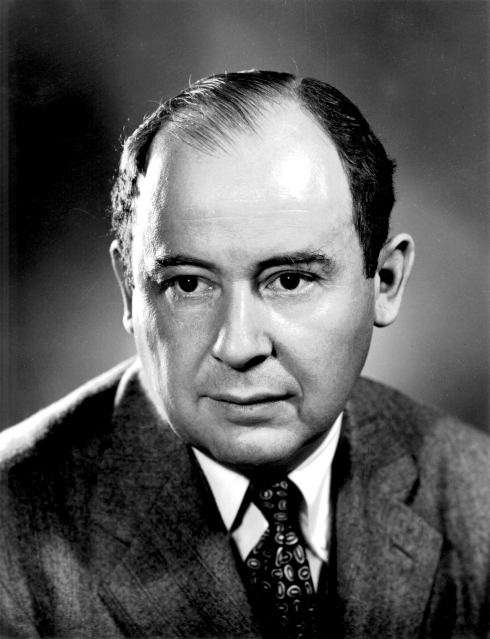
\includegraphics[width=\textwidth]{Pics/john-von-neumann}

John von Neumann
\end{columns}
\end{frame}


\begin{frame}{D\&C og Merge Sort}
\begin{itemize}
 \item Divide and Conquer almennt:
 \begin{itemize}
  \item \textbf{Divide:} Skipta verkefninu upp í undirverkefni sem eru minna tilvik af upphaflega verkefninu
  \item \textbf{Conquer:} Leysa vandamálin endurkvæmt þar til þau eru af viðráðanlegri stærð, þá eru þau leyst á auðveldan hátt
  \item \textbf{Combine:} Sameina lausnir undirverkefnanna til að mynda lausn á 
 \end{itemize}
 \item Divide and Conquer í Merge Sort: 
 \begin{itemize}
  \item \textbf{Divide:} $n$ staka inntakinu er skipt upp í tvo $n/2$ staka undirlista
  \item \textbf{Conquer:} Nota Merge Sort á undirlistana þar til þeir eru af lengd 1, og þ.a.l. sjálfkrafa í réttri röð
  \item \textbf{Combine:} Sameina undirlistana í raðaðan heildarlista
 \end{itemize}
\end{itemize}
\end{frame}

\begin{frame}{Hvað er í gangi?}
\vspace{-0.1\textheight}
\begin{center}
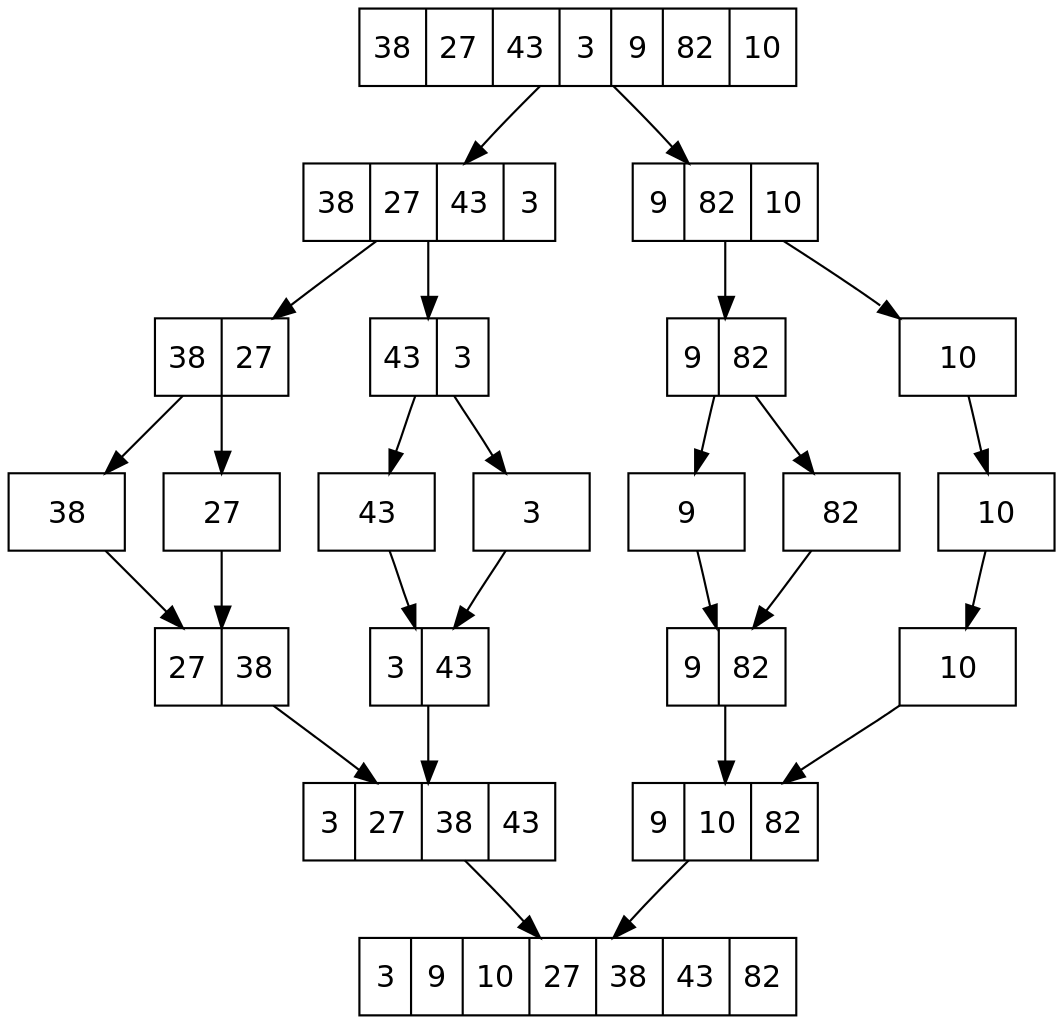
\includegraphics[height=0.8\textheight]{Pics/merge-sort-diagram}
\end{center}
\end{frame}

\begin{frame}{Merge Sort}
Endurkvæm útfærsla á Merge Sort reikniritinu
\begin{center}
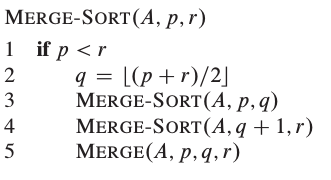
\includegraphics[scale=0.5]{Pics/merge-sort}
\end{center}
Hér eru $p$ og $r$ vísar í listanum. Í upphafi er kallað á fallið með \texttt{merge\_sort(A,1,n)}, þar sem $n$ er lengd listans.
\end{frame}

\begin{frame}{YouTube}
\url{http://www.youtube.com/watch?v=ZRPoEKHXTJg}
\end{frame}

\begin{frame}{Endurbætur á merge sort}
\begin{itemize}
 \item Samhliða vinnsla
 \begin{itemize}
  \item Sameining undirlista er að vissu leyti óháð sameiningu annarra lista 
 \end{itemize}
 \item Notkun Insertion Sort í vissum tilfellum\ldots
 \begin{itemize}
  \item \ldots á stutta undirlista?
  \item \ldots á undirlista sem eru nær raðaðir?
  \item Vinsæl útfærsla: Timsort
 \end{itemize}
 \item Önnur skipting en tvískipting?
\end{itemize}
\end{frame}

\begin{frame}{Quicksort}
\pause
\begin{columns}[c]
\column{0.7\textwidth}
Quicksort er mikið notað reiknirit með eftirfarandi eiginleika:
\begin{itemize}
 \item Ekki stöðugt (e. \emph{stable})
 \item $O(\log(n))$ auka minni
 \item Oftast $O(n\log(n))$ keyrslutími ($O(n^2)$ í versta tilfellinu)
 \item Ekki ``adaptive''
\end{itemize}
Oft mjög hagkvæmt við raunverulegar aðstæður.
\column{0.3\linewidth}
\begin{center}
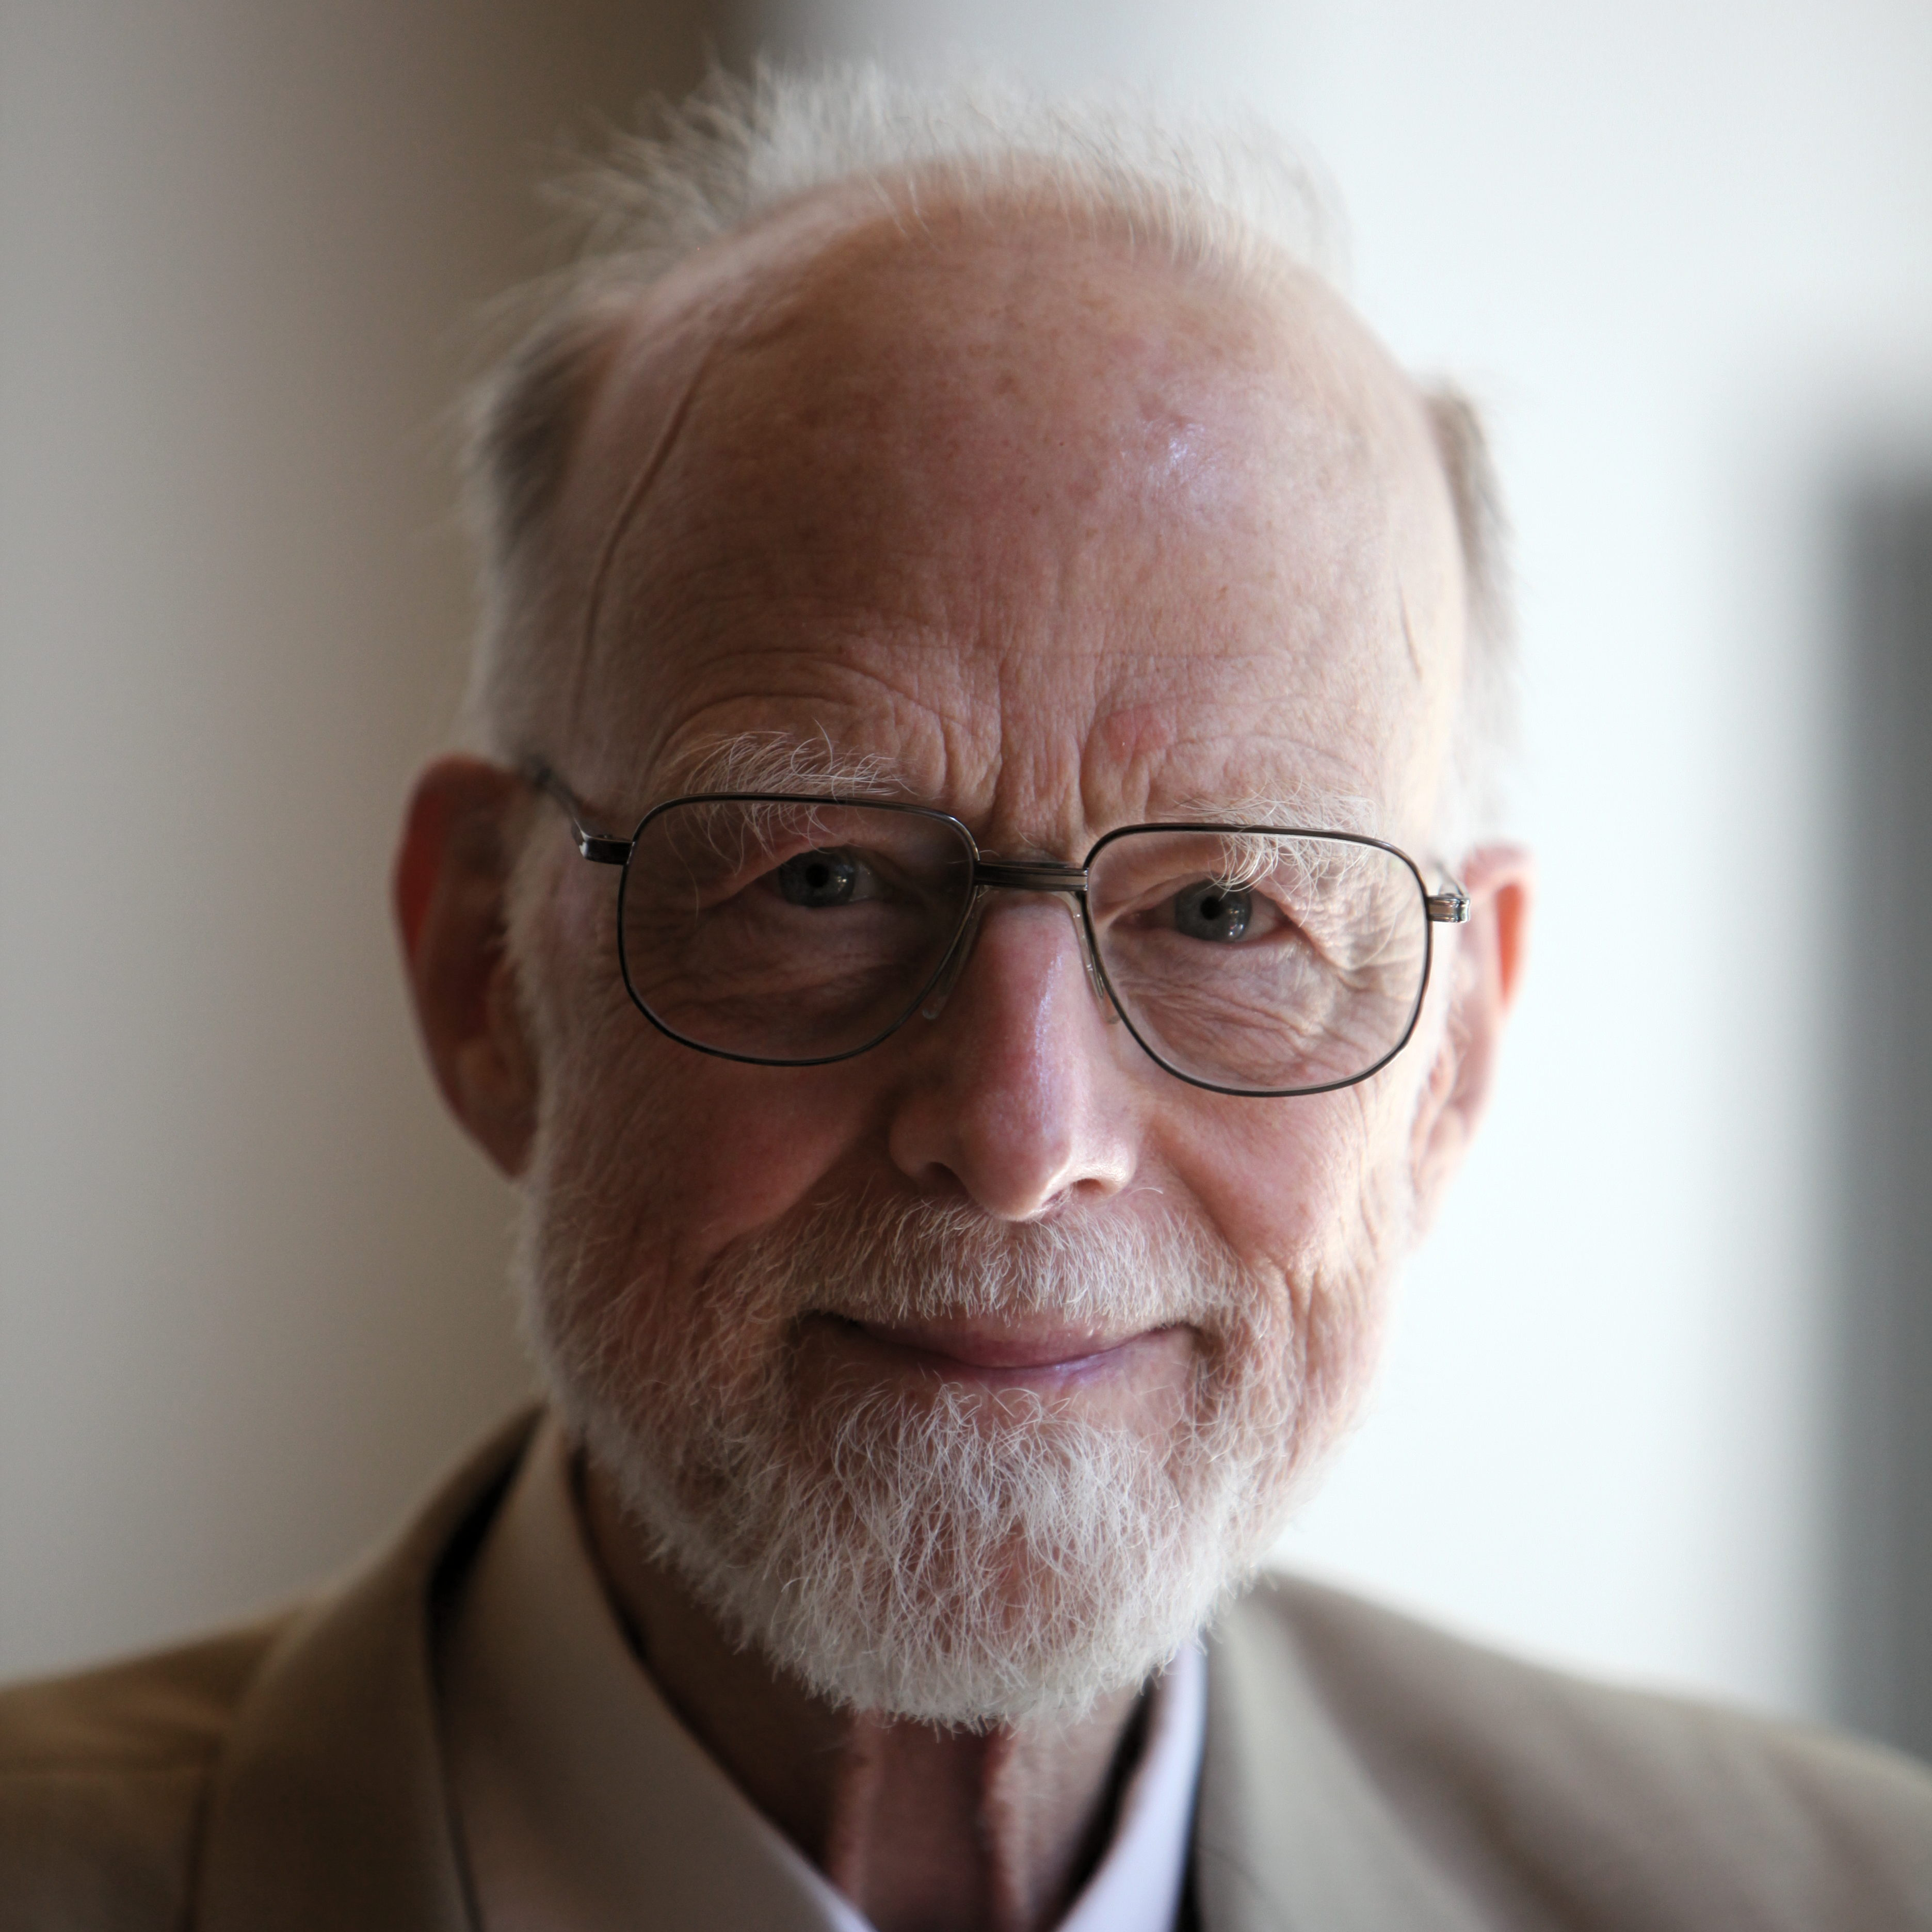
\includegraphics[width=\textwidth]{Pics/Hoare}
\end{center}
Tony Hoare fann upp Quicksort árið 1960
\end{columns}
\end{frame}

\begin{frame}{Divide and Conquer}
Lýsum Quicksort á eftirfarandi hátt:
\begin{itemize}
  \item \textbf{Divide:} Skiptum listanum (e. \emph{partition the list)} $A[p \ldots r]$ upp í tvo undirlista. Finnum stak $A[q]$ í listanum. Látum undirlistana vera $A[p \ldots q-1]$ og $A[q + 1 \ldots r]$ og skiptum á stökum svo að hvert stak í fyrri listanum sé minna en eða jafnt $A[q]$ og að hvert stak í seinni listanum sé stærra en eða jafnt $A[q]$.
  \item \textbf{Conquer:} Röðum undirlistunum $A[p \ldots q-1]$ og $A[q + 1 \ldots r]$ með endurkvæmri notkun Quicksort.
  \item \textbf{Combine:} Ekki nauðsynlegt, þar sem röðun hvers einasta undirlista þýðir að allur listinn er sjálfkrafa í réttri röð.
\end{itemize}
\end{frame}

\begin{frame}[fragile]{Quicksort}
Útfærsla á Quicksort reikniritinu sjálfu er tiltölulega einföld.
\begin{verbatim}
Quicksort(A,p,r)
if p < r
  q = partition(A, p, r)
  Quicksort(A, p, q - 1)
  Quicksort(A, q + 1, r)
\end{verbatim}
Hér eru $p$ og $r$ vísar í listanum. Í upphafi er kallað á fallið með \verb|Quicksort(A,1,n)|, þar sem $n$ er lengd listans.

Galdurinn er því greinilega í \verb|partition| fallinu. (Líkt og hann er í \verb|merge| fallinu í Merge Sort)
\end{frame}

\begin{frame}[fragile]{Partition - möguleg útfærsla}
Þetta \verb|partition| fall tekur inn lista $A$ ásamt vísum $p$ og $r$ svo að $A[p \ldots r]$ sé undirlisti.
\begin{verbatim}
partition(A, p, r)
  x = A[r] // x is pivot
  i = p - 1
  for j = p to r - 1
    if A[j] <= x
      i = i + 1
      swap A[i], A[j]
   swap A[i + 1], A[r]
   return i + 1
\end{verbatim}
\end{frame}

\begin{frame}{Dæmi um keyrslu Partition}
\begin{center}
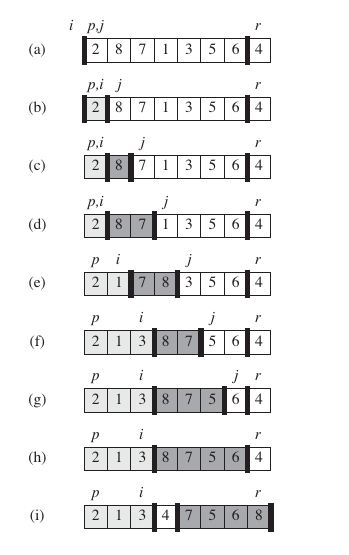
\includegraphics[height=0.9\textheight]{Pics/Quicksort}
\end{center}
\end{frame}

\begin{frame}{YouTube}
\url{http://www.youtube.com/watch?v=9IqV6ZSjuaI}
\end{frame}

\begin{frame}{Tímaflækja Quicksort}
Lausleg greining:
\begin{itemize}
  \item \emph{Í versta tilfellinu} skiptir partition-fallið hverjum lista í lista af stærð 0 og $n-1$. Slík skipting tekur $O(n)$ tíma og þarf að framkvæma $O(n)$ sinnum.
  \item \emph{Í besta tilfellinu} er skiptingin jöfn. Skiptingin tekur enn $O(n)$ tíma, en helmingunin á lengd listanna minnkar fjölda skiptinga sem þarf að framkvæma (niður í $O(\log(n))$.
\end{itemize}
Athugum að valið á pivot-staki skv. reikniritinu á fyrri glæru framkallar verstu skiptinguna við for-röðuð gögn (eða öfug gögn).
\end{frame}

\begin{frame}{Val á Pivot-staki}
Lykillinn að góðri Quicksort-útfærslu liggur í vali á Pivot-staki. Skoðum algenga möguleika:
\begin{itemize}
 \item Slembið (e. \emph{Random}) stak
 \item Miðstakið
 \item Median-of-three (Mo3)
 \begin{itemize}
  \item First, last, middle
  \item 3 random
 \end{itemize}
\end{itemize}
\end{frame}

\begin{frame}{Raunverulegur hraði}
\begin{itemize}
 \item Quicksort er þekkt fyrir góða frammistöðu miðað við önnur röðunarreiknirit. Tvær ástæður:
 \begin{itemize}
  \item Fastarnir sem stóra-O felur
  \item ``Locality of reference''
 \end{itemize}
\end{itemize}
\end{frame}

\begin{frame}{Samanburður}
\href{https://www.youtube.com/watch?v=ZZuD6iUe3Pc}{Nokkur röðunarreiknirit borin saman}
\end{frame}


\end{document}
